% Adjust these for the path of the theme and its graphics, relative to this file
%\usepackage{beamerthemeFalmouthGamesAcademy}
\usepackage{../../beamerthemeFalmouthGamesAcademy}
\usepackage{multimedia}
\graphicspath{ {../../} }

% Default language for code listings
\lstset{language=C++,
        morekeywords={each,in,nullptr}
}

% For strikethrough effect
\usepackage[normalem]{ulem}
\usepackage{wasysym}

\usepackage{pdfpages}

\usepackage{circuitikz}

% http://www.texample.net/tikz/examples/state-machine/
\usetikzlibrary{arrows,automata}
\usetikzlibrary{calc}

\iftoggle{printable}{
    \newcommand{\circuitcolour}{black}
}{ % else
    \newcommand{\circuitcolour}{white}
}

\newcommand{\modulecode}{COMP260}\newcommand{\moduletitle}{Distributed Systems}\newcommand{\sessionnumber}{5}

\begin{document}
\title{\sessionnumber: Logic and memory}
\subtitle{\modulecode: \moduletitle}

\frame{\titlepage} 

\begin{frame}{Worksheet 4}
    \begin{center} 
        Due \textbf{next Friday!}
    \end{center}
\end{frame}

\part{Scholarly literature}
\frame{\partpage}

\begin{frame}{Scholarly work}
	\begin{itemize}
		\pause\item What is a ``scholarly'' work?
		\pause\item How do we know if something is scholarly?
	\end{itemize}
\end{frame}

\usetikzlibrary{shapes,arrows,intersections}
\usetikzlibrary{matrix,fit,calc,trees,positioning,arrows,chains,shapes.geometric,shapes}

\begin{frame}{Pyramid of sources}
	\centering
	\begin{tikzpicture}
	\coordinate (A) at (-4.5,0) {};
	\coordinate (B) at ( 4.5,0) {};
	\coordinate (C) at (0,5*1.2) {};
	\path[name path=AC,draw=none] (A) -- (C);
	\path[name path=BC,draw=none] (B) -- (C);
	\iftoggle{printable}{
		\filldraw[draw=Purple, ultra thick,fill=Purple!10!White] (A) -- (B) -- (C) -- cycle ;
	}{ % else
		\filldraw[draw=Purple, ultra thick,fill=Purple!10!Black] (A) -- (B) -- (C) -- cycle ;
	}	

	\foreach \y/\A in {4.5/{Scholarly journals and conference proceedings},
					   4.0/{Scholarly books and book chapters},
					   3.5/{Masters and PhD theses},
					   3.0/{Government documents, trade books and white papers},
					   2.5/{Specialised magazines},
					   2.0/{Pre-print papers (e.g.\ arXiv)},
					   1.5/{General interest books, magazines and newspapers},
					   1.0/{General encyclop\ae dias},
					   0.5/{Websites, blogs, Wikipedia},
					   0.0/{Online discussion boards, personal communications}
					} {
		\pause
		\path[draw=none, very thick, dashed, name path=horiz] (A|-0,\y*1.2) -- (B|-0,\y*1.2);
		\draw[draw=Purple, very thick, dashed, 
			  name intersections={of=AC and horiz,by=P},
			  name intersections={of=BC and horiz,by=Q}] (P) -- (Q)
			  %node[midway,above,font=\bfseries\scshape,color=red!60!Brown] {\A};
			  node[midway,above] {\A};
	}
	\end{tikzpicture}
\end{frame}

\begin{frame}{Appropriateness of sources}
	\pause It is important to question the \textbf{appropriateness} of sources you use in academic work
	\begin{itemize}
		\pause\item \textbf{Validity}: Are claims based upon a correct interpretation of the evidence?
		\pause\item \textbf{Rigor}: Was the method of collecting evidence appropriate to ensure 
			comprehensive coverage while also avoiding bias?
	\end{itemize}
\end{frame}

\begin{frame}{Appropriateness of sources}
	\begin{itemize}
		\pause\item \textbf{Reliability}: has the claim been replicated, or at least reviewed, by other academics?
		\pause\item \textbf{Authoritativeness}: do we know who the author is?
			Does the author have enough experience in the field to present a fair and balanced argument?
		\pause\item \textbf{Venue}: Is the publisher reputable and free of undue editorial influences?
	\end{itemize}
\end{frame}

\begin{frame}{Appropriateness of sources}
	\pause There are of course exceptions where sources are presented as \textbf{artefacts} and/or \textbf{archives}:
	\begin{itemize}
		\pause\item Citing a newspaper as evidence for a claim based on the reception of a new technology
		\pause\item Citing a manufacturer's technical manual when describing a technical feature of a platform
		\pause\item Citing a Reddit post by a well-known industry figure as evidence for expert opinion
	\end{itemize}
	\pause The \textbf{way} in which sources are \textbf{used} is therefore important
\end{frame}

\part{Library resources}
\frame{\partpage}

\begin{frame}{Library catalogue}
	\begin{center}
		\url{http://library.fxplus.ac.uk/}
	\end{center}
\end{frame}

\begin{frame}{Web proxy}
	Insert \texttt{.ezproxy.falmouth.ac.uk} at the end of the \textbf{domain name}
		(before the \texttt{/})
	\pause
	\begin{center}
		\texttt{http://www.example.com/example/page.html}
		
		\pause $\downarrow$
		
		\texttt{http://www.example.com\uline{.ezproxy.falmouth.ac.uk}/ example/page.html}
	\end{center}
\end{frame}

\begin{frame}{ACM Digital Library}
	\begin{center}
		\small\url{http://dl.acm.org.ezproxy.falmouth.ac.uk/}
	\end{center}
\end{frame}

\begin{frame}{IEEE Xplore}
	\begin{center}
		\small\url{http://ieeexplore.ieee.org.ezproxy.falmouth.ac.uk/}
	\end{center}
\end{frame}

\begin{frame}{GDC Vault}
	\begin{center}
		\small\url{http://www.gdcvault.com.ezproxy.falmouth.ac.uk/}
		
		\vspace{2ex}
		
		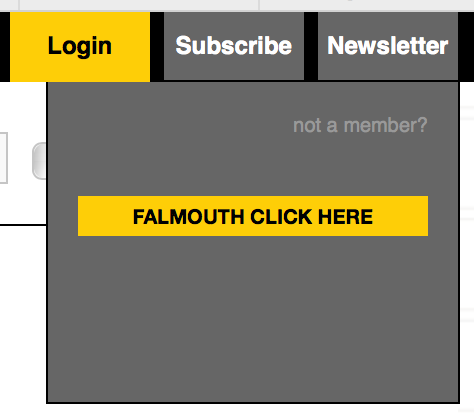
\includegraphics[width=0.4\textwidth]{gdc_login}
	\end{center}
\end{frame}

\begin{frame}{Ethics of paywalls}
	\begin{itemize}
		\pause\item Is it ethical for publishers to charge for access to publicly-funded academic research?
		\pause\item Many journals offer free \textbf{open access}
			\begin{itemize}
				\pause\item Some high quality, some low quality...
			\end{itemize}
		\pause\item Many authors put papers on their \textbf{personal websites}
			\begin{itemize}
				\pause\item Some publishers allow this, others turn a blind eye
			\end{itemize}
		\pause\item Sites like \textbf{sci-hub} aim to be a ``Pirate Bay for papers''
	\end{itemize}
\end{frame}

\part{Referencing}
\frame{\partpage}

\begin{frame}{Which referencing style?}
	\begin{itemize}
		\pause\item Many different referencing styles exist
		\pause\item Most Falmouth courses use \textbf{Harvard} style
		\pause\item In Computing we tend to prefer \textbf{IEEE} style
		\pause\item If assignments specify which one to use then use it
		\pause\item Otherwise choose whichever you prefer --- just be \textbf{consistent}
		\pause\item Tools like BibTeX make it easy to switch styles
	\end{itemize}
\end{frame}

\begin{frame}{Direct quotations}
	\begin{itemize}
		\pause\item \textbf{THIS IS IMPORTANT:} \#1 source of alleged academic misconduct cases for the Research Journal!
		\pause\item If you are directly quoting a source, you must make it \textbf{very clear} that this is the case
		\pause\item Common convention is to use \textbf{quotation marks and italics}, with a citation straight after ---
			\textit{``To be or not to be, that is the question''} [Shakespeare 1604]
		\pause\item Direct quotations are generally bad style in technical writing --- better to rephrase, summarise, synthesise key points
		\pause\item Most written assignments at Falmouth are passed through TurnItIn --- plagiarism \textbf{will} be detected!
	\end{itemize}
\end{frame}

\begin{frame}{IEEE referencing style}
	\begin{center}
		\small\url{https://ieeeauthorcenter.ieee.org/wp-content/uploads/IEEE-Reference-Guide.pdf}
	\end{center}
\end{frame}

\begin{frame}{Harvard referencing style}
	\begin{center}
		\small\url{https://studyhub.fxplus.ac.uk/study-guides/referencing/harvard-referencing-falmouth-university}
	\end{center}
\end{frame}

\begin{frame}{BibTeX entry types}
	\begin{center}
		\small\url{https://en.wikibooks.org/wiki/LaTeX/Bibliography_Management\#BibTeX}
	\end{center}
\end{frame}

\begin{frame}{Writing BibTeX entries}
	\begin{itemize}
		\pause\item Some websites provide pre-written BibTeX entries for papers
		\pause\item Beware of copying and pasting these as they are often incomplete, incorrectly formatted or just wrong!
		\pause\item You must \textbf{always} check your bibliography in the compiled PDF and fix any errors
		\pause\item You \textbf{will} lose marks on your written assignments otherwise!
	\end{itemize}
\end{frame}


\part{Logic gates}
\frame{\partpage}

\newcommand{\TT}{\textsc{True}}
\newcommand{\FF}{\textsc{False}}
\newcommand{\OP}[1]{\ \textsc{#1}\ }
\newcommand{\OPand}{\OP{and}}
\newcommand{\OPor}{\OP{or}}
\newcommand{\OPxor}{\OP{xor}}
\newcommand{\OPnand}{\OP{nand}}
\newcommand{\OPnor}{\OP{nor}}
\newcommand{\OPxnor}{\OP{xnor}}
\newcommand{\OPnot}{\textsc{not}\ }

\newcommand{\OPname}{}
\newcommand{\OPenglishA}{}
\newcommand{\OPenglishB}{}
\newcommand{\OPtable}{}
\newcommand{\OPdiagram}{}

\newcommand{\OPframe}[5]{
	\begin{frame}{#1}
		\pause
		\begin{center}
			#2 \par if and only if \par #3
		\end{center}
		\pause
		\begin{columns}
			\begin{column}{0.48\textwidth}
				\begin{center}
					#4
				\end{center}
			\end{column}
			\pause
			\begin{column}{0.48\textwidth}
				\begin{center}
					\begin{circuitikz} \draw[color=\circuitcolour]
						#5
					\end{circuitikz}
				\end{center}
			\end{column}
		\end{columns}
	\end{frame}
}

\begin{frame}{Boolean logic}
	\begin{itemize}
		\pause\item Works with two values: \TT\ and \FF
		\pause\item Foundation of the \textbf{digital computer}:
			represented in circuits as \textbf{on} and \textbf{off}
		\pause\item Representing as $1$ and $0$ leads to \textbf{binary notation}
		\pause\item One boolean value = one \textbf{bit} of information
		\pause\item Programmers use boolean logic for conditions in \lstinline{if} and \lstinline{while}
			statements
	\end{itemize}
\end{frame}

%\begin{frame}{Simulating logic circuits}
	%\centering
	%\url{http://logic.ly/demo/}
%\end{frame}

\OPframe{Not}
	{$\OPnot A$ is \TT}{$A$ is \FF}
	{\begin{tabular}{|c||c|} \hline
		$A$ & $\OPnot A$ \\\hline
		\FF & \TT \\
		\TT & \FF \\\hline
	\end{tabular}}
	{ (0,0) node[not port] (gate) {}
	(gate.in)  node[anchor=east] {$A$}
	(gate.out) node[anchor=west] {$\OPnot A$}
	; }

\OPframe{And}
	{$A \OPand B$ is \TT}{\textbf{both $A$ and $B$} are \TT}
	{\begin{tabular}{|c|c||c|}
		\hline
		$A$ & $B$ & $A \OPand B$ \\\hline
		\FF & \FF & \FF \\
		\FF & \TT & \FF \\
		\TT & \FF & \FF \\
		\TT & \TT & \TT \\\hline
	\end{tabular}}
	{ (0,0) node[and port] (gate) {}
	(gate.in 1) node[anchor=east] {$A$}
	(gate.in 2) node[anchor=east] {$B$}
	(gate.out)  node[anchor=west] {$A \OPand B$}
	; }

\OPframe{Or}
	{$A \OPor B$ is \TT}{\textbf{either $A$ or $B$, or both,} are \TT}
	{\begin{tabular}{|c|c||c|}
		\hline
		$A$ & $B$ & $A \OPand B$ \\\hline
		\FF & \FF & \FF \\
		\FF & \TT & \TT \\
		\TT & \FF & \TT \\
		\TT & \TT & \TT \\\hline
	\end{tabular}}
	{ (0,0) node[or port] (gate) {}
	(gate.in 1) node[anchor=east] {$A$}
	(gate.in 2) node[anchor=east] {$B$}
	(gate.out)  node[anchor=west] {$A \OPor B$}
	; }

\begin{frame}{Socrative \texttt{FALCOMPED}}
	What is the value of
	$$ A \OPand (B \OPor C) $$
	when
	\begin{align*}
		A &= \TT \\
		B &= \FF \\
		C &= \TT
	\end{align*}
	?
\end{frame}

\begin{frame}{Socrative \texttt{FALCOMPED}}
	What is the value of
	$$ (\OPnot A) \OPand (B \OPor C) $$
	when
	\begin{align*}
		A &= \TT \\
		B &= \FF \\
		C &= \TT
	\end{align*}
	?
\end{frame}

\begin{frame}{Socrative \texttt{FALCOMPED}}
	For what values of $A, B, C, D$ is
	$$ A \OPand \OPnot B \OPand \OPnot (C \OPor D) = \TT $$
	?
\end{frame}

\begin{frame}{Socrative \texttt{FALCOMPED}}
	What is the value of
	$$ A \OPor \OPnot A $$
	?
\end{frame}

\begin{frame}{Socrative \texttt{FALCOMPED}}
	What is the value of
	$$ A \OPand \OPnot A $$
	?
\end{frame}

\begin{frame}{Socrative \texttt{FALCOMPED}}
	What is the value of
	$$ A \OPor A $$
	?
\end{frame}

\begin{frame}{Socrative \texttt{FALCOMPED}}
	What is the value of
	$$ A \OPand A $$
	?
\end{frame}

\begin{frame}{Socrative \texttt{FALCOMPED}}
	What expression is equivalent to this circuit?
	\begin{center}
		\begin{circuitikz} \draw[color=\circuitcolour]
			(0,0) node[and port] (gateA) {}
			(0,-2) node[or port] (gateB) {}
			(1,0) node[not port] (gateC) {}
			(3.5,-1) node[or port] (gateD) {}
			(gateA.out) -- (gateC.in) {}
			(gateC.out) -| (gateD.in 1) {}
			(gateB.out) -| (gateD.in 2) {}
			(gateD.out) node[anchor=west] {?}
			(gateA.in 1) node[anchor=east] {$A$}
			(gateA.in 2) node[anchor=east] {$B$}
			(gateB.in 1) node[anchor=east] {$C$}
			(gateB.in 2) node[anchor=east] {$D$}
			;
		\end{circuitikz}
	\end{center}
\end{frame}

\begin{frame}[fragile]{Writing logical operations}
	\pause
	\centering
	\begin{tabular}{|c||c|c|c|}
		\hline
		Operation & Python & C family & Mathematics \\\hline
		$\OPnot A$
			& \texttt{not a}
			& \texttt{!a}
			& $\neg A$ {\huge\phantom{$I$}} or {\huge\phantom{$I$}} $\overline{A}$
			\pause\\
		$A \OPand B$ 
			& \texttt{a and b}
			& \texttt{a \&\& b}
			& $A \wedge B$
			\pause\\
		$A \OPor B$ 
			& \texttt{a or b}
			& \texttt{a || b}
			& $A \vee B$
			\\\hline
	\end{tabular}
	\pause
	\par\vspace{2ex}\par
	Other operators can be expressed by combining these
\end{frame}

\begin{frame}{De Morgan's Laws}
	\pause
	$$ \OPnot (A \OPor B) = (\OPnot A) \OPand (\OPnot B) $$
	\pause
	$$ \OPnot (A \OPand B) = (\OPnot A) \OPor (\OPnot B) $$
	\pause
	Proof: Worksheet 4, questions 3a and 3b
\end{frame}

\part{Truth tables}
\frame{\partpage}

\begin{frame}{Enumeration}
	\begin{itemize}
		\pause\item Since booleans have only two possible values, we can often \textbf{enumerate}
			all possible values of a set of boolean variables
		\pause\item For $n$ variables there are $2^n$ possible combinations
		\pause\item Essentially, all the $n$-bit binary numbers
		\pause\item A \textbf{truth table} enumerates all the possible values of a boolean expression
		\pause\item Can be used to prove that two expressions are equivalent
	\end{itemize}
\end{frame}

\begin{frame}{Truth table example}
	$$ (A \OPor \OPnot B) \OPand C $$
	\begin{centering}
	    \small
		\begin{tabular}{|ccc|cc|c|}
		    \hline
			$A$ & $B$ & $C$ & $\OPnot B$ & $A \OPor \OPnot B$ & $(A \OPor \OPnot B) \OPand C$ \\\hline\pause
			\FF & \FF & \FF & \TT & \TT & \FF \\\pause
			\FF & \FF & \TT & \TT & \TT & \TT \\\pause
			\FF & \TT & \FF & \FF & \FF & \FF \\\pause
			\FF & \TT & \TT & \FF & \FF & \FF \\\pause
			\TT & \FF & \FF & \TT & \TT & \FF \\\pause
			\TT & \FF & \TT & \TT & \TT & \TT \\\pause
			\TT & \TT & \FF & \FF & \TT & \FF \\\pause
			\TT & \TT & \TT & \FF & \TT & \TT \\\hline
		\end{tabular}
	\end{centering}
\end{frame}

\part{Other logic gates}
\frame{\partpage}

\OPframe{Exclusive Or}
	{$A \OPxor B$ is \TT}{\textbf{either $A$ or $B$, but not both,} are \TT}
	{\begin{tabular}{|c|c||c|}
		\hline
		$A$ & $B$ & $A \OPand B$ \\\hline
		\FF & \FF & \FF \\
		\FF & \TT & \TT \\
		\TT & \FF & \TT \\
		\TT & \TT & \FF \\\hline
	\end{tabular}}
	{ (0,0) node[xor port] (gate) {}
	(gate.in 1) node[anchor=east] {$A$}
	(gate.in 2) node[anchor=east] {$B$}
	(gate.out)  node[anchor=west] {$A \OPxor B$}
	; }

\begin{frame}{Socrative \texttt{FALCOMPED}}
	How can $A \OPxor B$ be written using the operations $\OPand, \OPor, \OPnot$?
\end{frame}

\begin{frame}
    \begin{center}
        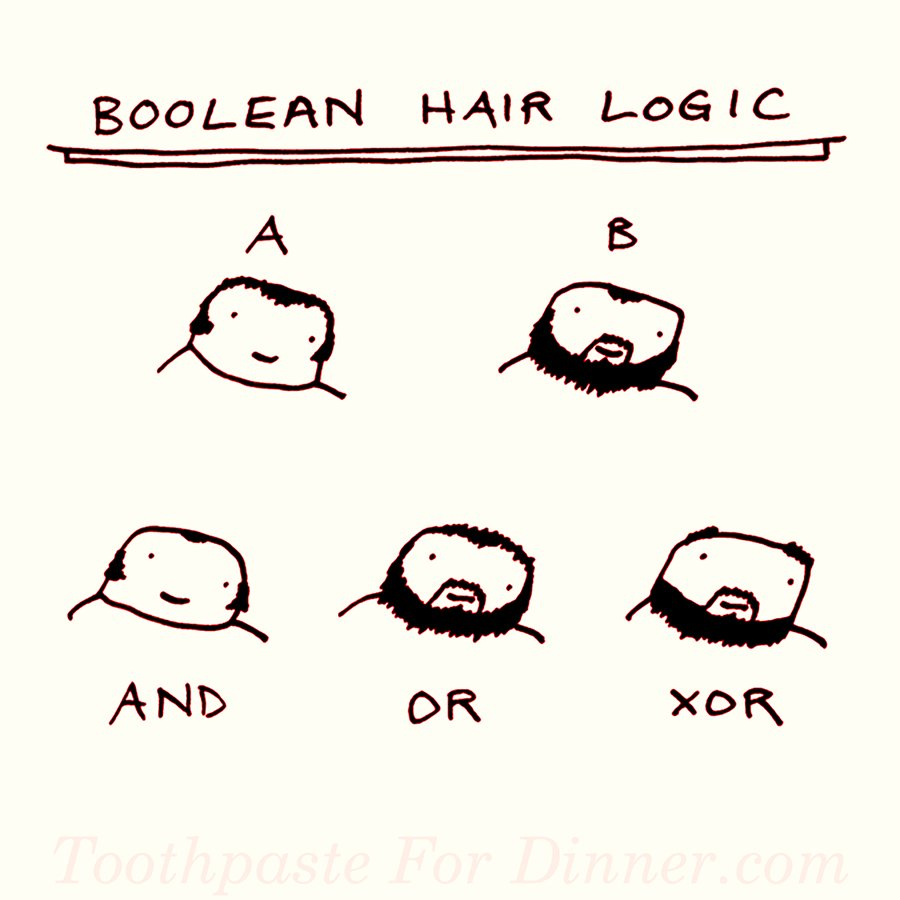
\includegraphics[width=0.8\textwidth]{boolean_hair_logic}
    \end{center}
\end{frame}

\begin{frame}{Negative gates}
	\pause
	\begin{center}
		$\OPnand, \OPnor, \OPxnor$ \par are the \textbf{negations} of \par $\OPand, \OPor, \OPxor$
	\end{center}
	\pause
	\begin{columns}
		\begin{column}{0.48\textwidth}
			\begin{center}
				\begin{align*}
					A \OPnand B &= \OPnot (A \OPand B) \\
					A \OPnor B &= \OPnot (A \OPor B) \\
					A \OPxnor B &= \OPnot (A \OPxor B)
				\end{align*}
			\end{center}
		\end{column}
		\pause
		\begin{column}{0.48\textwidth}
			\begin{center}
				\begin{circuitikz} \draw[color=\circuitcolour]
					(0,0) node[nand port] (gate) {}
					(gate.in 1) node[anchor=east] {$A$}
					(gate.in 2) node[anchor=east] {$B$}
					(gate.out)  node[anchor=west] {$A \OPnand B$}
					;
				\end{circuitikz}
				\begin{circuitikz} \draw[color=\circuitcolour]
					(0,0) node[nor port] (gate) {}
					(gate.in 1) node[anchor=east] {$A$}
					(gate.in 2) node[anchor=east] {$B$}
					(gate.out)  node[anchor=west] {$A \OPnor B$}
					;
				\end{circuitikz}
				\begin{circuitikz} \draw[color=\circuitcolour]
					(0,0) node[xnor port] (gate) {}
					(gate.in 1) node[anchor=east] {$A$}
					(gate.in 2) node[anchor=east] {$B$}
					(gate.out)  node[anchor=west] {$A \OPxnor B$}
					;
				\end{circuitikz}
			\end{center}
		\end{column}
	\end{columns}
\end{frame}

\begin{frame}{Any logic gate can be constructed from NAND gates}
    \begin{center}
        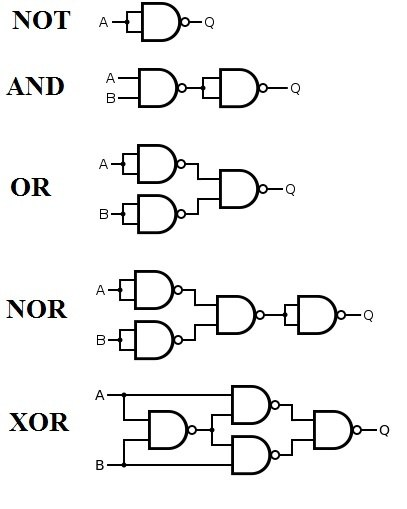
\includegraphics[height=0.7\textheight]{nand_gates}
    \end{center}
\end{frame}

\begin{frame}{What does this circuit do?}
	\centering
	\begin{circuitikz} \draw[color=\circuitcolour]
		(0,0) node[nand port] (gateA) {}
		(0,-2) node[nand port] (gateB) {}
		(gateA.out) -- ($ (gateA.out) + (0, -0.5) $) -- ($ (gateB.in 1) + (0, 0.5) $) -- (gateB.in 1) {}
		(gateB.out) -- ($ (gateB.out) + (0, 0.5) $) -- ($ (gateA.in 2) + (0, -0.5) $) -- (gateA.in 2) {}
		(gateA.out) -- ($ (gateA.out) + (0.5, 0) $) node[anchor=west] {$Q$}
		(gateB.out) -- ($ (gateB.out) + (0.5, 0) $) node[anchor=west] {$\overline{Q}$}
		(gateA.in 1) -- ($ (gateA.in 1) + (-0.5, 0) $) node[anchor=east] {$S$}
		(gateB.in 2) -- ($ (gateB.in 2) + (-0.5, 0) $) node[anchor=east] {$R$}
		;
	\end{circuitikz}
	\begin{itemize}
		\pause\item This is called a \textbf{NAND latch}
		\pause\item It ``remembers'' a single boolean value
		\pause\item Put a few billion of these together
			(along with some control circuitry)
			and you've got \textbf{memory}!
	\end{itemize}
\end{frame}

\begin{frame}{NAND gates}
    \begin{itemize}
        \pause\item All arithmetic and logic operations, as well as memory, can be built from NAND gates
        \pause\item So an entire computer can be built just from NAND gates!
        \pause\item Play the game: \url{http://nandgame.com}
        \pause\item NAND gate circuits are \textbf{Turing complete}
        \pause\item The same is true of NOR gates
    \end{itemize}
\end{frame}


\part{Arithmetic Logic Unit}
\frame{\partpage}

\begin{frame}{Arithmetic Logic Unit}
	\begin{center}
		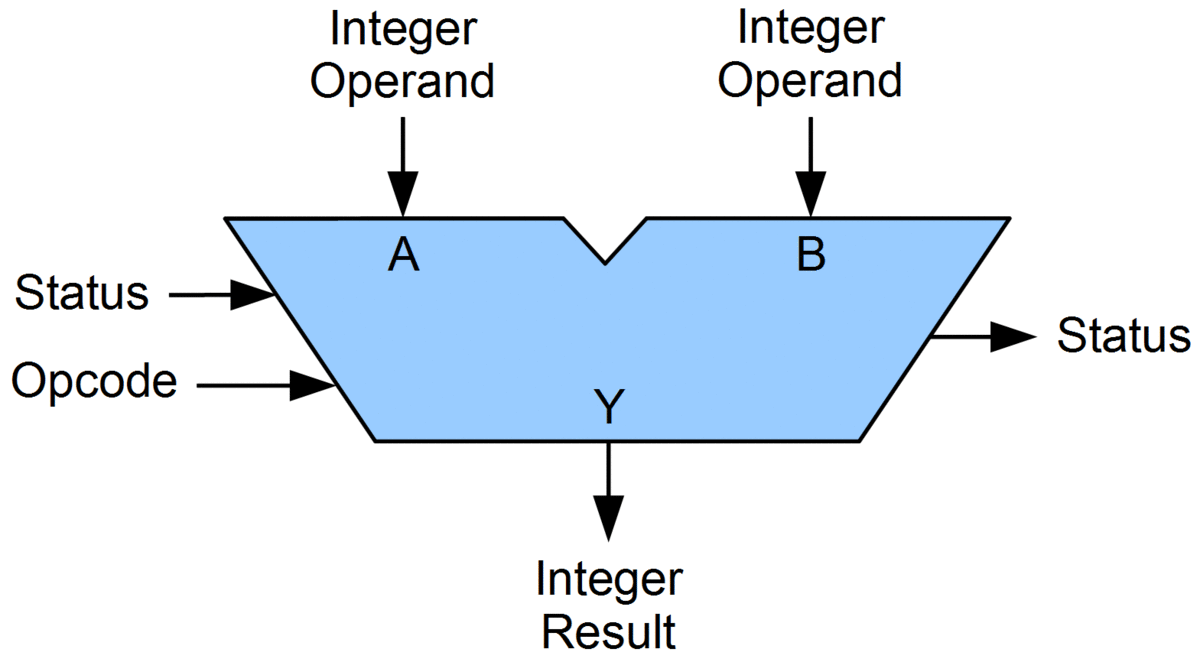
\includegraphics[width=\textwidth]{alu}
		%https://commons.wikimedia.org/wiki/File:ALU_block.gif
	\end{center}
\end{frame}

\begin{frame}{Arithmetic Logic Unit}
	\begin{itemize}
		\pause\item Important part of the CPU
		\pause\item Inputs:
			\begin{itemize}
				\item \textbf{Operand} words $A, B$
				\item \textbf{Opcode}
				\item \textbf{Status} bits
			\end{itemize}
		\pause\item Outputs:
			\begin{itemize}
				\item \textbf{Result} word $Y$
				\item \textbf{Status} bits
			\end{itemize}
		\pause\item Opcode specifies how $Y$ is calculated based on $A$ and $B$
	\end{itemize}
\end{frame}

\begin{frame}{ALU operations}
	Typically include:
	\begin{itemize}
		\pause\item Add with carry
		\pause\item Subtract with borrow
		\pause\item Negate (2's complement)
		\pause\item Increment, decrement
		\pause\item Bitwise \textsc{and}, \textsc{or}, \textsc{not}, $\dots$
		\pause\item Bit shifts
	\end{itemize}
\end{frame}

\newcommand{\carry}[1]{\uncover<#1->{$_1$}}
\newcommand{\nocarry}[1]{\phantom{$_1$}}

\begin{frame}{Addition with carry}
	In base 10:
	\begin{center}
		\begin{tabular}{lllll}
			& 1 & 2 & 3 & 4 \\
			+ & 5\nocarry{4} & 6\carry{3} & 7\carry{2} & 8\nocarry{1} \\\hline
			& \uncover<5->{6} & \uncover<4->{9} & \uncover<3->{1} & \uncover<2->{2}
		\end{tabular}
	\end{center}
\end{frame}

\begin{frame}{Addition with carry}
	In base 2:
	\begin{center}
		\fbox{$1 + 1 = 10$ \qquad $1 + 1 + 1 = 11$}
		
		\vspace{2ex}
		
		\begin{tabular}{lllllllll}
			& 0 & 1 & 1 & 0 & 1 & 1 & 1 & 0 \\
			+ &
				0\carry{8} &
				0\carry{7} &
				1\nocarry{6} &
				0\carry{5} &
				0\carry{4} &
				1\carry{3} &
				1\nocarry{2} &
				1 \\\hline
			&
				\uncover<9->{1} &
				\uncover<8->{0} &
				\uncover<7->{0} &
				\uncover<6->{1} &
				\uncover<5->{0} &
				\uncover<4->{1} &
				\uncover<3->{0} &
				\uncover<2->{1}
		\end{tabular}
	\end{center}
\end{frame}

\begin{frame}{1-bit adder}
	\begin{center}
		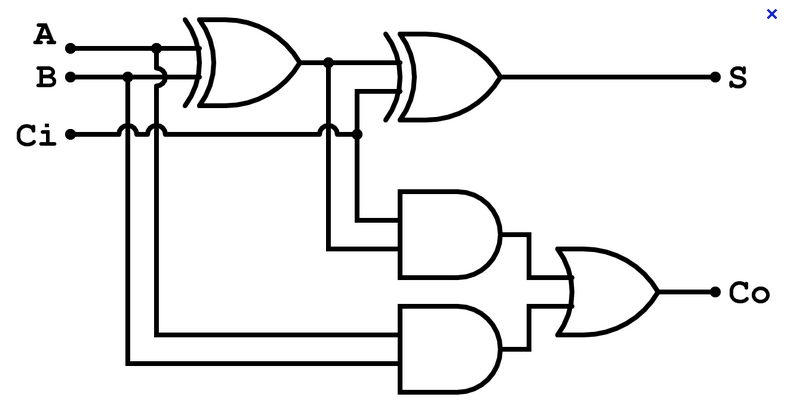
\includegraphics[width=\textwidth]{1bit_adder}
	\end{center}
\end{frame}

\begin{frame}{$n$-bit adder}
	\begin{center}
		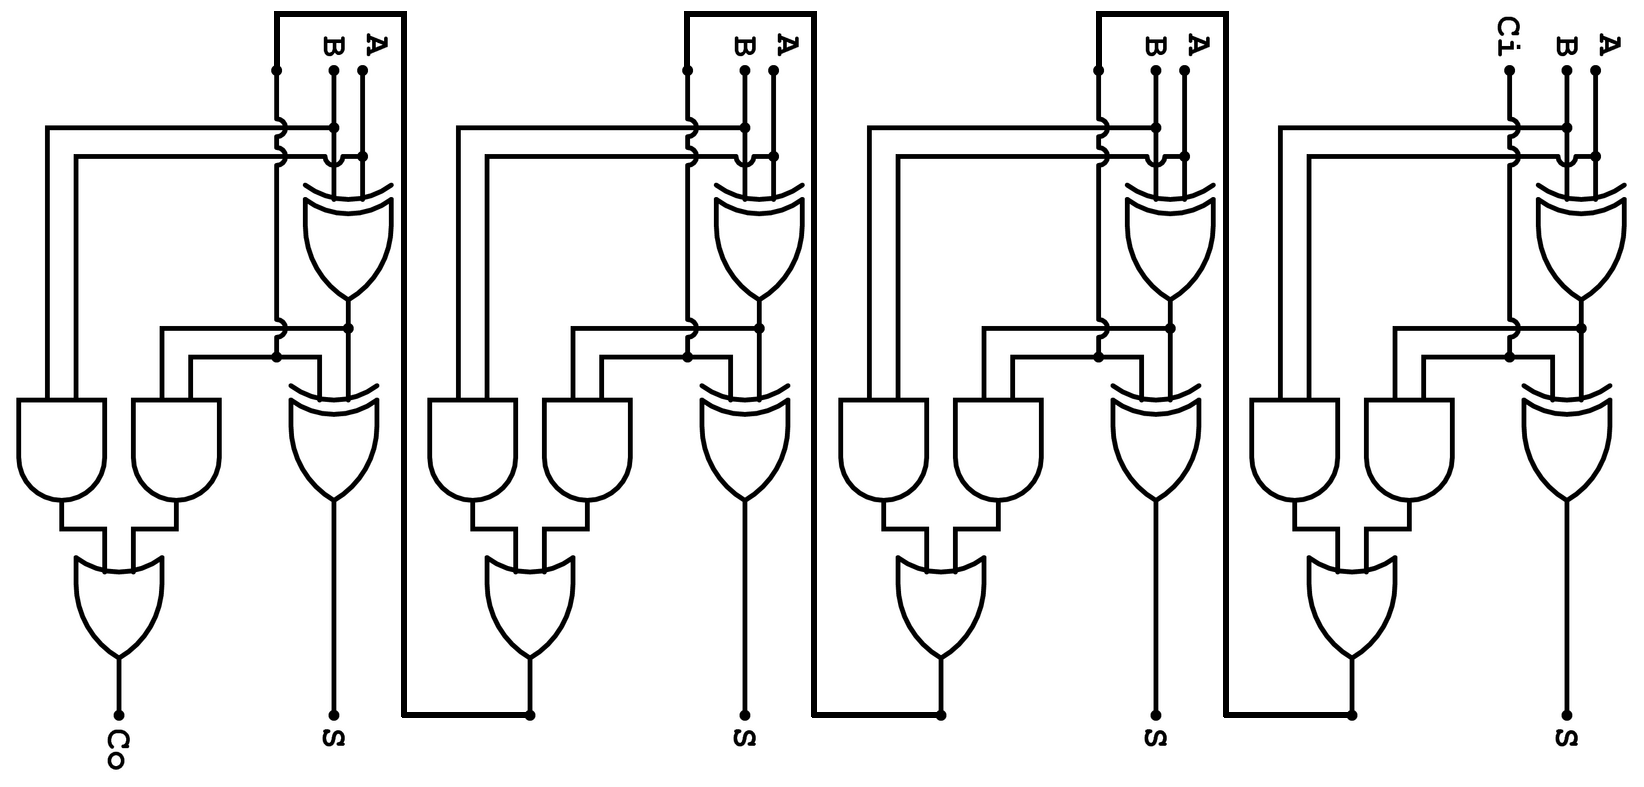
\includegraphics[width=\textwidth]{nbit_adder}
	\end{center}
\end{frame}



\end{document}
